%!TEX root = ../main.tex
\chapter{Introduction}
Complex oxides are a unique class of materials exhibiting a large number of technologically relevant functional properties including ferroelectricity, superconductivity, and ferromagnetism ~\cite{Cohen1992,Liang1992,Rao2000}.  
These functional properties are intimately linked to the spin, charge, lattice, and orbital degrees of freedom resulting in extreme sensitivity to external stimuli, structural distortions, and chemical doping.  
Advances in thin film growth techniques have enabled the growth of epitaxial thin films with atomically flat interfaces, allowing for the creation of artificial multi-layered structures with novel interfacial behavior.  
\section{Perovskite Structure}
One class of complex oxides, the perovskites, have received a wide range of interest due to their intriguing functional properties.  
Perovskite oxides have the general chemical formula \ce{ABO3}.  
In an ideal case they can be constructed by placing a \ce{BO6} octahedron at the center of a cubic lattice and then filling the corner positions with A-site cations, resulting in a 3 dimensional network of corner sharing \ce{BO6} octahedra.  
A 2x2x2 perovskite supercell is shown in Figure~\ref{fig:perovskite_unitcell}.  
\begin{figure}[tb]
    \centering
    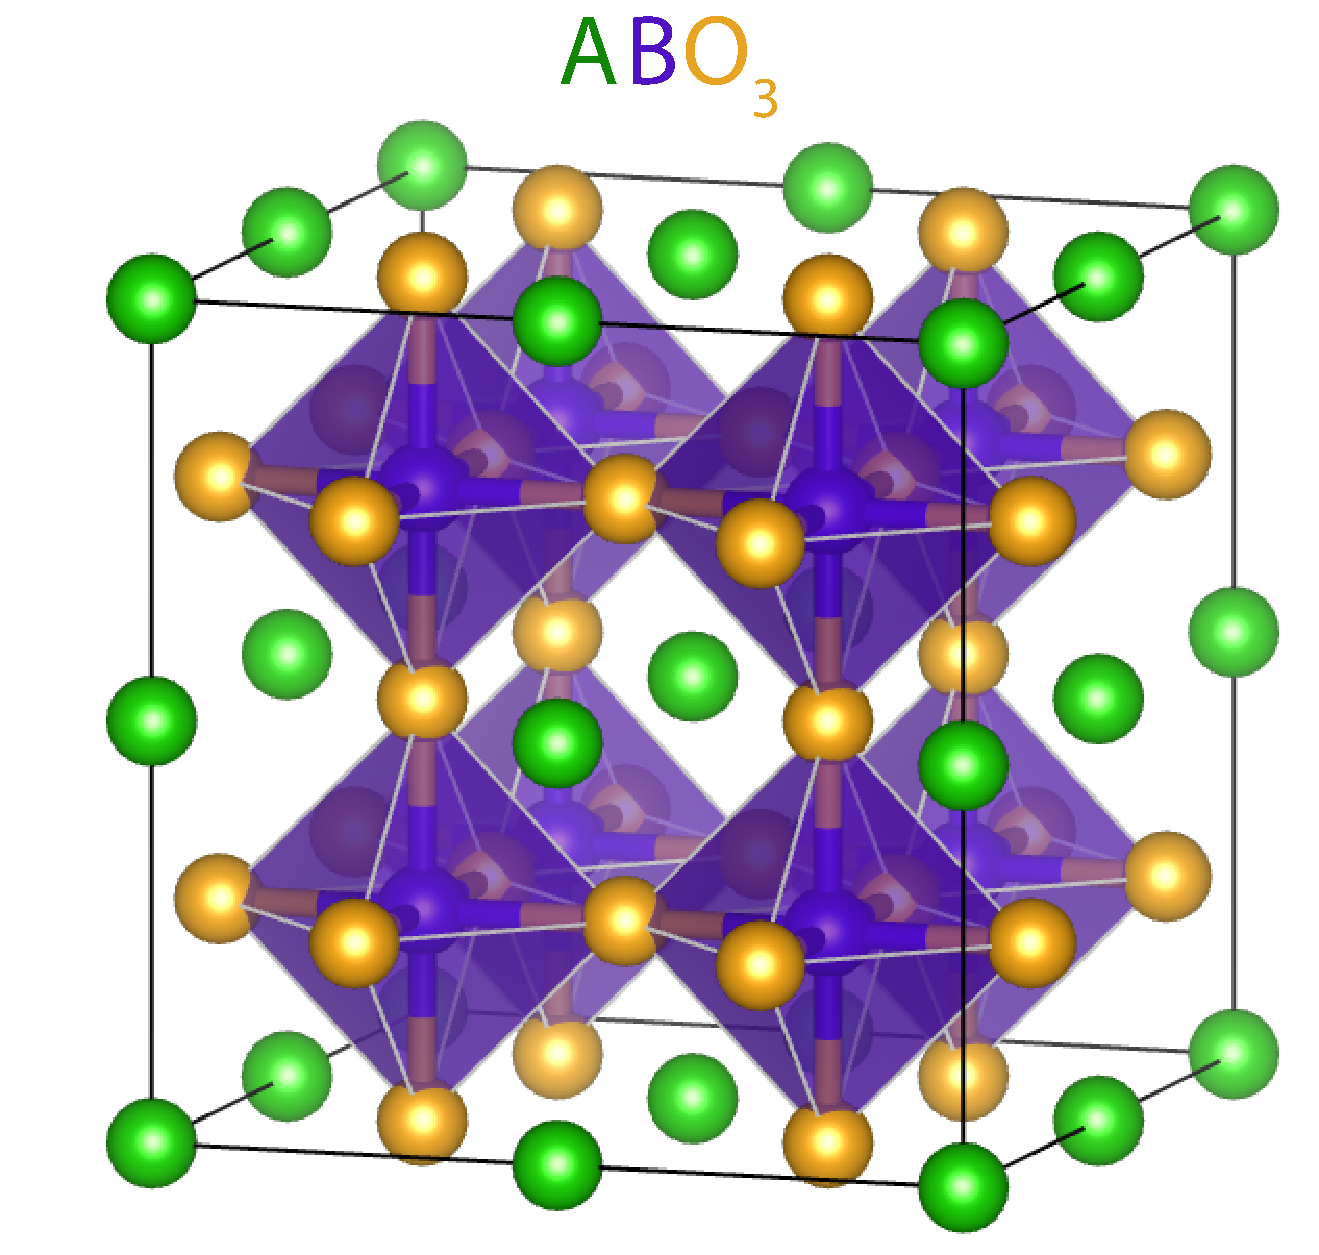
\includegraphics[width=.35\textwidth]{figures/intro/Perovskite_supercell.pdf}
    \caption[Perovskite crystal structure]{8 unit cells of the perovskite structure, illustrating the \ce{BO6} octahedra as the primary building block}
    \label{fig:perovskite_unitcell}
\end{figure}
Unique to perovskites is their ability to host nearly the entire periodic table in the various atomic positions.  
Figure~\ref{fig:intro/perovskite_ptable} depicts which atoms can be placed in the perovskite structure clearly illustrating the chemical diversity of the A and B sites.  
\begin{figure}[tb]
    \centering
    \includegraphics[width=.5\textwidth]{figures/intro/PerovskitePTable.png}
    \caption[Elements that can exist in the perovskite structure]{Color coded periodic table depicting which elements can sit in the respective positions in the perovskite crystal structure.  A-site ions are green, B-site ions are purple, and O-sites are gold. \cite{Petrovic2015}}
    \label{fig:intro/perovskite_ptable}
\end{figure}
This ability to host so many atoms is a direct result of the flexible corner shared \ce{BO6} octahedral network that is able to both distort and rotate to accommodate varying ion sizes.  
The Goldschmidt tolerance factor relates the A-O and B-O bond lengths, dictating whether or not specific A and B site ions can be accommodated~\cite{Goldschmidt1926}:
\begin{equation}
    t = \frac{r_A + r_O}{\sqrt{2}\left(r_B + r_O\right)}
    \label{eq:Goldschmidt}
\end{equation}
where $r_A$, $r_B$, and $r_O$ are the ionic radii of the various ions.  
For the ideal structure with cubic symmetry, $t=1$.  
The perovskite structure remains stable for values of $t$ ranging from 0.78 to 1.05 with symmetry lowering distortions occurring for values differing from unity, resulting in orthorhombic, rhombohedral, and hexagonal perovskite variants~\cite{Vailionis2015}.  
The tolerance factor summarizes the changing of B-O-B bond angles and bond lengths needed to accommodate larger or smaller ions and codifies the resulting crystallographic symmetry changes.  

While the Goldschmidt tolerance factor describes the resulting symmetry in a perovskite, it contains no information about the actual changes in the \ce{BO6} octahedral network.  
Changes to the B-O-B bond angle can also be described as rotations of the \ce{BO6} octahedra away from their ideal positions.  
Effort has been made to describe all of the possible rotation patterns of \ce{BO6} octahedra in perovskites, with the only constraint being the corner connectivity between octahedra.  
In the early 1970s, Glazer studied all of the possible rotation patterns and determined that there are only 23 distinct possibilities that can be described with a succinct three index notation~\cite{Glazer1972,Glazer1975}.  
Consider Figure~\ref{fig:inpahse_oop_octahedral}, which compares the $\mathrm{a}^0\mathrm{a}^0\mathrm{c}^+$ and $\mathrm{a}^0\mathrm{a}^0\mathrm{c}^-$ octahedral rotation patterns.  
\begin{figure}[b]
    \centering
    \includegraphics[width=.5\textwidth]{figures/intro/rondinelli_inphase_oophase.png}
    \caption[Depiction of in-phase and out-of-phase octahedral rotations]{Comparison of in-phase rotations (left) and out-of-phase rotations (right) about the c-axis.  \cite{Rondinelli2012}}
    \label{fig:inpahse_oop_octahedral}
\end{figure}
In this notation, each index refers to rotations about the three principle axes and the superscript denotes whether the rotations are in-phase (+), out-of-phase (-), or non-existent (o).  
If two indices have the same letter that means that the rotation magnitude is equal around those two axes.  
Figure~\ref{fig:inpahse_oop_octahedral} depicts the difference between in-phase and out-of-phase octahedral rotations.  
If the rotations are out-of-phase, the sign of rotation changes in each unit cell, whereas it remains the same for in-phase rotations.  
Two of the most common octahedral rotation patterns are the rhombohedral $\mathrm{a}^-\mathrm{a}^-\mathrm{a}^-$ pattern occurring due to ordered rotations about the [111] direction, and the orthorhombic $\mathrm{a}^-\mathrm{b}^+\mathrm{a}^-$pattern caused by rotations about the [110] direction.  

The presence of octahedral tilts changes the overall crystalline symmetry of the perovskite structure.
It can be helpful to consider a ``pseudocubic'' (pc) set of axes and lattice parameters that correspond to the ideal perovskite perovskite building blocks.  
Transformation from an orthorhombic unit cell to a pseudocubic unit cell can be performed through a simple transformation, with the relationship between orthorhombic and low index pseudocubic directions outlined in Table~\ref{tab:ortho pc transform}.  
The pseudocubic representation in Table~\ref{tab:ortho pc transform} is just one of multiple different transformation that can be used for orthorhombic unit cells.  
\begin{table}[tb!]
\centering
\caption{Relationship between low index pseudocubic and orthorhombic directions for a (110) oriented orthorhombic substrate, where the listed pseudocubic directions are parallel to the original orthorhombic directions}
\label{tab:ortho pc transform}
\begin{tabular}{@{}ll@{}}
\toprule
Orthorhombic & Pseudocubic\\ \midrule
\hkl[1 1 0] & \hkl[0 0 1] \\
\hkl[1 -1 0] & \hkl[0 1 0] \\
\hkl[0 0 2] & \hkl[1 0 0] \\
\bottomrule
\end{tabular}
\end{table}


\section{Magnetism in Perovskites}
Magnetic behavior in materials is due to exchange interactions between two neighboring atoms with net magnetic moments.  
Magnetic exchange interactions are effectively a driving force minimizing energy when spins are aligned in antiparallel or parallel directions, depending on the sign of the exchange interaction.  
Multiple types of exchange interactions exist: direct exchange in which two atoms are in close proximity and interact directly with one another, and indirect exchange which requires an intermediary to facilitate the exchange interaction between separated atoms~\cite{Spaldin2010}.    
In the perovskite structure, the A site ion typically has a full shell electrical configuration and thus the magnetic behavior can be solely attributed to the B site ion.  
The large separation between neighboring B site ions requires an indirect exchange mechanism mediated by the \ce{O^2-} ions to account for any observed (anti)ferromagnetic behavior.  

Consider the perovskite \ce{La_{0.7}Sr_{0.3}MnO3} (LSMO) which consists of a mixture of La and Sr ions on the A site, and Mn on the B site, and is ferromagnetic below \SI{370}{\kelvin}~\cite{Hemberger2002}.  
A direct result of two A site ions with different valence is that the Mn ion exists with both \ce{Mn^3+} and \ce{Mn^4+} states in an equal proportion to the \ce{Sr}/\ce{La} ratio assuming complete oxygenation.  

When a transition metal such as \ce{Mn} is octahedrally coordinated with oxygen ions, overlap between the metal 3d orbitals and oxygen 2p orbitals is significant, and the energy associated with this overlap is known as the crystal-field stabilization energy (CFSE)~\cite{Rohrer2001}.  
Two d-orbitals, $d_{z^2}$ and $d_{x^2-y^2}$, point directly at the surrounding oxygen ligands and are destabilized, while the other three d-orbitals, $d_{xy}$, $d_{yx}$, and $d_{zx}$, point at the space in between atoms and become stabilized.  
As a result, the five fold degeneracy of the 3d orbitals is lifted forming a triply degenerate set of $t_{2g}$ orbitals and a doubly degenerate set of $e_g$ orbitals.  
A schematic for this splitting due to ligand field effects is shown in Figure~\ref{fig:cfse_d_orbital}.  
\begin{figure}[tb]
    \centering
    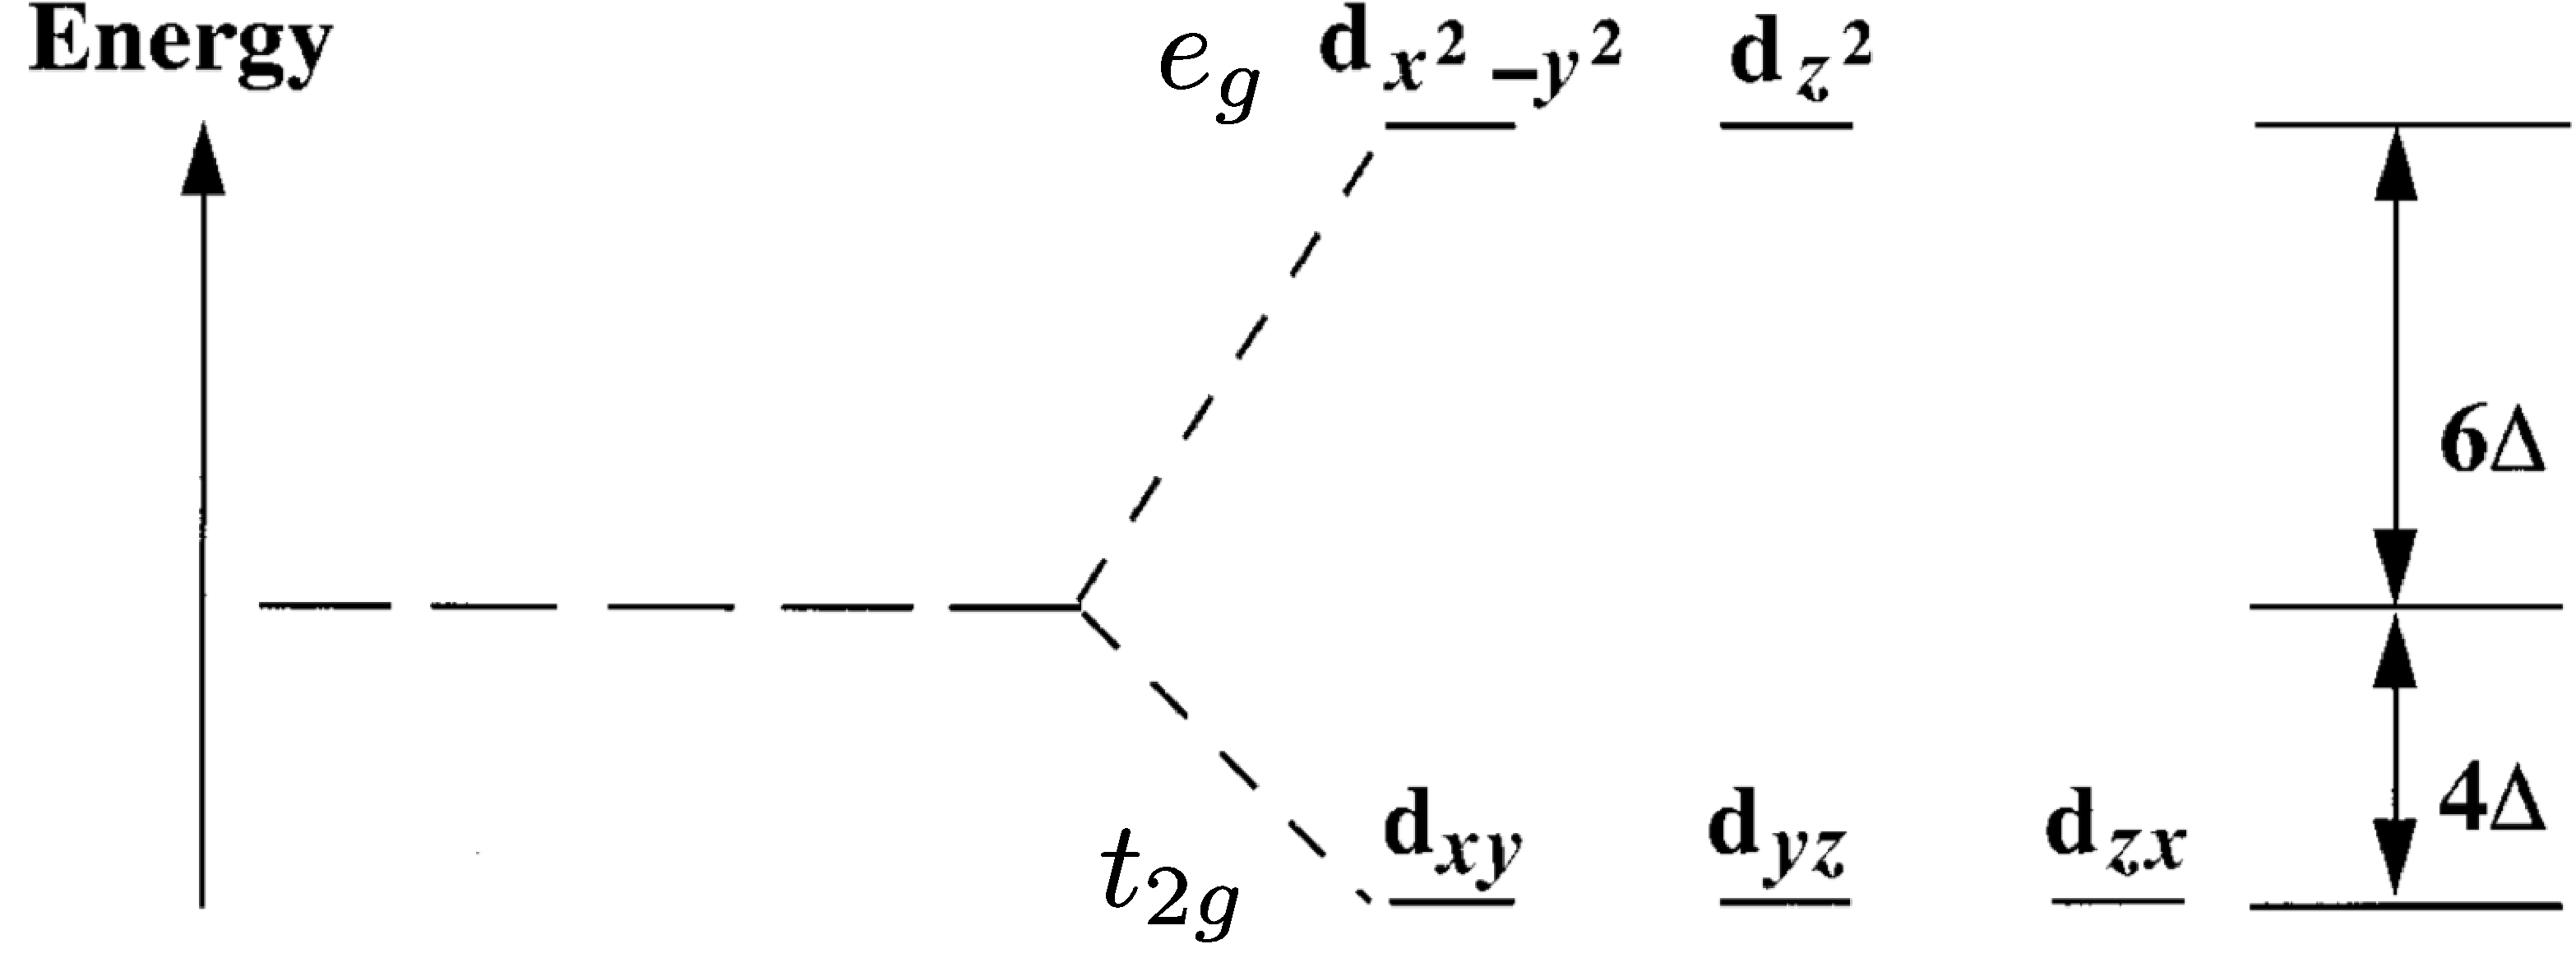
\includegraphics[width=.7\textwidth]{figures/intro/cfse_rohrer.pdf}
    \caption[Octahedral crystal field splitting of 3d orbitals]{CFSE splitting of 3d-orbitals in an octahedral bonding environment. \cite{Rohrer2001}}
    \label{fig:cfse_d_orbital}
\end{figure}
The separation between $t_{2g}$ and $e_g$ orbitals is typically on the order of 1-2 \si{\eV} in manganites, but is significantly lower for cobaltites~\cite{Fujioka2015}.  

When electrons fill the $t_{2g}$ and $e_g$ orbitals, they obey Hund's rules which state that electrons prefer to maximize the total angular momentum and total spin of an orbital.  
In other words, the lowest energy state exists when electrons fill different orbitals with parallel spin configurations.  
The case for \ce{Mn^3+} and \ce{Mn^4+} ions is illustrated in Figure~\ref{fig:Mn_double_exchange}.  
\ce{Mn} ions with different valence on either side of an intermediate O ion can now interact indirectly: first, an electron from an O 2p orbital hops onto a neighboring \ce{Mn^4+} ion followed by an electron hopping from the \ce{Mn^3+} ion to the now partially filled O 2p orbital~\cite{Zener1951}.  
Because there is an energy penalty associated with flipping electron spins, the spin direction is preserved and ferromagnetic behavior is realized.  
\begin{figure}[t]
    \centering
    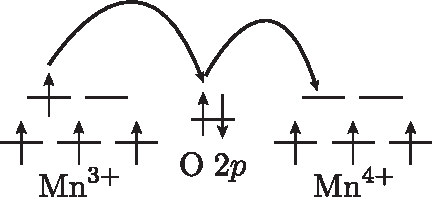
\includegraphics[width=.65\textwidth]{figures/intro/Mn_dub_exchange_schematic.pdf}
    \caption[Schematic for double exchange mechanism in LSMO between \ce{Mn^3+} and \ce{Mn^4+} ions]{Schematic for double exchange mechanism in LSMO between \ce{Mn^3+} and \ce{Mn^4+} ions.  First, an electron hops from the O 2p orbital to an empty orbital in the \ce{Mn^4+} ion maintaining spin alignment following Hund's rules.  Next, an electron hops from the \ce{Mn^3+} ion to the now partially empty O 2p orbital.  Spin direction is preserved during this hopping process, and the two ion positions have been switched.}
    \label{fig:Mn_double_exchange}
\end{figure}
Since electrons are physically hopping between neighboring ions, the onset of ferromagnetism via the double exchange mechanism is also coincident with the onset of metallic behavior.  
Furthermore, the rate and probability of electron hopping depends sensitively on the overlap between B 3d and O 2p orbitals and magnetism is therefore strongly linked with the B-O-B bond geometry and the octahedral tilt pattern.  

Another type of indirect exchange interaction that can occur in perovskites is the superexchange mechanism.  
Consider two \ce{Mn^3+} ions located on either side of an oxygen ion with a \SI{180}{\degree} bond angle, illustrated in Figure~\ref{fig:mn_superexchange}.  
\begin{figure}[h]
    \centering
    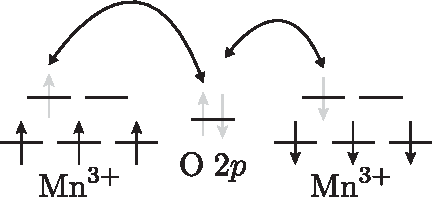
\includegraphics[width=.65\textwidth]{figures/intro/Mn_superexchange_schematic.pdf}
    \caption[Schematic for superexchange in \ce{LaMnO3}]{Schematic for superexchange in \ce{LaMnO3}.  Virtual electron hopping occurs from the O 2p orbital to neighboring Mn 3d orbitals (indicated by grey arrows).  Spin direction is preserved in this virtual hop leading to antiferromagnetic behavior.}
    \label{fig:mn_superexchange}
\end{figure}
A virtual hop from the oxygen 2p orbital to the Mn 3d orbital can occur on either side of the oxygen ion and, since the oxygen 2p orbital interacting with neighboring Mn 3d orbitals is completely filled, the electrons hopping to either Mn ion will have an opposite spin direction.  
Consequently the spin direction on the two Mn ions will be antiparallel resulting in antiferromagnetic behavior and because the hopping process is virtual the sample is insulating.  
The superexchange mechanism is dependent on orbital filling and bonding geometry: for \SI{180}{\degree} bonds the interaction is antiferromagnetic while for \SI{90}{\degree} bonds it is ferromagnetic~\cite{Bhattacharya2014}.  
The rules for determining the resulting magnetic behavior have been codified by Goodenough, Kanamori, and Anderson~\cite{Anderson1950}.  

\section{\texorpdfstring{\ce{La_{1-x}Sr_{x}MnO3}}{La(1-x)SrxMnO3} and \texorpdfstring{\ce{La_{1-x}Sr_{x}CoO3}}{La(1-x)SrxCoO3}}
Thin films and heterostructures of Sr-doped \ce{LaMnO3} and \ce{LaCoO3} will be the main focus of this work.  
Introduction of $x$ moles of the bivalent dopant Sr into either of these compounds results in the formation of an equimolar amount of \ce{Mn^4+} (\ce{Co^4+}) ions resulting in a mixed 3+ / 4+ valence state and the onset of ferromagnetism via the double exchange mechanism.  
The large number of unique phases present in the \ce{La_{1-x}Sr_{x}MnO3} temperature - doping phase diagram in Figure~\ref{fig:lsmo_phase} illustrates the complex interplay between spin, orbit, lattice, and charge degrees of freedom in this material.  
Figure~\ref{fig:lsmo_phase} also depicts the changing crystalline symmetry as the concentration of \ce{Sr} is changed: the ionic radii of Sr, \SI{1.31}{\angstrom}, is slightly larger than that of La, \SI{1.22}{\angstrom}~\cite{Shannon1976}.  
In order to accommodate this change, the \ce{BO6} octahedra rotate and the symmetry changes from orthorhombic to rhombohedral, followed by tetragonal and hexagonal symmetries as the value of $x$ increases.  
\begin{figure}[tb!]
    \centering
    \includegraphics[width=.5\textwidth]{figures/intro/LSMOPhase.png}
    \caption[\ce{La_{1-x}Sr_{x}MnO3} phase diagram]{\ce{La_{1-x}Sr_{x}MnO3} Sr-doping-temperature phase diagram.  \textbf{crystal structure} O: Jahn-Teller distorted orthorhombic, O': orthorhombic, O'': orbital-ordered orthorhombic, R: Rhombohedral, T: tetragonal, Mc: monoclinic, H: hexagonal, \textbf{magnetic order} PM: paramagnetic, CA: canted, yellow: antiferromagnetic, Blue: ferromagnetic, \textbf{electronic state} I: insulating, M: metallic.  \cite{Hemberger2002}}
    \label{fig:lsmo_phase}
\end{figure}
This work focuses on a doping concentration of \SI{0.3}{} where \ce{La_{0.7}Sr_{0.3}MnO3} (LSMO) is in a rhombohedral crystal structure and is a soft ferromagnetic metal with a low coercivity below a $T_c$ of \SI{370}{\kelvin}~\cite{Hemberger2002}.  

The doping-temperature phase diagram for \ce{La_{1-x}Sr_{x}CoO3} in Figure~\ref{fig:lsco_phase} shows similarities with that of \ce{La_{1-x}Sr_{x}MnO3}; however, distinct differences arise because \ce{La_{1-x}Sr_{x}CoO3} undergoes a phenomenon known as magnetoelectronic phase separation (MEPS) for low Sr-doping~\cite{Torija2011}.  
MEPS involves small ferromagnetic clusters that are embedded in a matrix of insulating antiferromagnetic material such that long range ferromagnetic order is not realized. 
Phase separated \ce{La_{1-x}Sr_{x}CoO3} exhibits glassy behavior and therefore this region of the phase diagram is denoted as a spin glass (SG).  
Long range ferromagnetism does not occur until the clusters grow in size and create a percolative network above $x=0.18$ upon which a metal-insulator transition occurs and long range ferromagnetism is realized.  
Furthermore the \ce{La_{1-x}Sr_{x}CoO3} phase diagram only covers doping concentrations from $x=0$ to $x=0.7$.  
At higher $x$ the perovskite structure is no longer the equilibrium phase and instead derivative structures are formed such as the oxygen deficient perovskite structure known as Brownmillerite~\cite{Jeen2013a}.  
\begin{figure}[h]
    \centering
    \includegraphics[width=.5\textwidth]{figures/intro/LSCO_Bulk_Phase_Wu2003_Labelled.eps}
    \caption[\ce{La_{1-x}Sr_{x}CoO3} phase diagram]{\ce{La_{1-x}Sr_{x}CoO3} composition - Sr-doping phase diagram.  SG = spin glass, PS = paramagnetic semiconductor, PM = paramagnetic metal, FM = ferromagnetic metal, MIT = metal-insulator transition, $T_{irr}$ = irreversiblity temperature, $T_{sst}$ = spin state transition temperature.  \cite{Wu2003}}
    \label{fig:lsco_phase}
\end{figure}
Another feature unique to \ce{La_{1-x}Sr_{x}CoO3} is the presence of spin state transitions.  
In this material the crystal field splitting between $e_g$ and $t_{2g}$ orbitals is small such that thermal energy can excite electrons from the $t_{2g}$ to $e_g$ orbitals.   
The presence of spin state transitions results in a diverse landscape of magnetic states~\cite{Wu2003}.  
The doping concentration of $x=0.3$ will be the focus of this study.  
At this Sr concentration, \ce{La_{0.7}Sr_{0.3}CoO3} (LSCO) is in a rhombohedral crystal structure and is a hard ferromagnet metal with a $T_c$ of \SI{210}{\kelvin}.  
Hard ferromagnets magnetically switch at larger fields than soft ferromagnets and typically have lower saturation magnetization.  

\section{Oxide Heterostructures}

Growing oxides into multilayered structures introduces another layer of complexity.  
The spin, charge, orbit, and lattice degrees of freedom vary dramatically across an interface and can lead to unexpected and difficult to predict physical behavior.  
One effect that occurs across an interface is the charge transfer of electrons from one material to another because of Fermi level ($E_F$) differences on either side of the interface.  
Electrons will travel into the material with the lower $E_F$ until the energy differences is equalized.  
The length scale for interfacial charge transfer is short in oxides, on the order of \SI{0.5}{\nm} to \SI{2}{\nm}, because oxides have a large dielectric constant and high carrier concentrations~\cite{Hellman2017}.  
As magnetic behavior is so closely linked with the valence state, charge transfer can drastically change local magnetic behavior.  
For example, interfacial ferromagnetism can be stabilized in nonmagnetic systems like in antiferromagnetic manganite superlattices~\cite{Santos2011} and \ce{LaNiO3} / \ce{CaMnO3} superlattices~\cite{Grutter2013}.  

Structural changes across interfaces can also influence the properties of an oxide heterostructure.  
When a thin film is grown on a substrate it can be strained depending on the relative lattice parameters and crystal structures of the substrate and thin film.  
Substrate-induced strain forces the in-plane lattice parameter of the film to match that of the substrate resulting in a tetragonally distorted film~\cite{Vailionis2011}.  
\ce{BO6} octahedral rotations are also modified by interfacial strain leading to a change in the B-O-B bond angles and a resultant impact on the magnetic behavior.  
Furthermore, \ce{BO6} octahedra are constrained to be corner connected, even across an interface, meaning that rotational patterns from a substrate can be induced into a film, providing yet another route in which magnetic behavior can be modified in oxide heterostructures.  
However, frequently, the rotation pattern observed in thin films differs both from that of the bulk material and of the substrate~\cite{Choquette2016}.  
Interestingly, the length scales over which interfacial strain and substrate induced rotational patterns persist differ~\cite{Rondinelli2012}.  

\section{LSMO / LSCO heterostructures}
\begin{sloppypar} % fixes LSAT chemical name extending to margins
Bilayers of LSMO and LSCO have been studied for their interesting magnetic switching behavior.  
When a hard ferromagnet (LSCO) and a soft ferromagnet (LSMO) are grown in a bilayer on \ce{(LaAlO3)_{0.3}(Sr2TaAlO6)_{0.7}} (LSAT) substrates, the major hysteresis loop showing the magnetization of the entire sample shows two distinct magnetic switching events~\cite{Li2014}.  
The black curve in Figure~\ref{fig:LSCO_LSMO_bilayer_loops} shows the magnetic switching behavior of a \SI{6}{\nm} LSMO / \SI{6}{\nm} LSCO bilayer on LSAT substrate.  
\begin{figure}[b!]
    \centering
    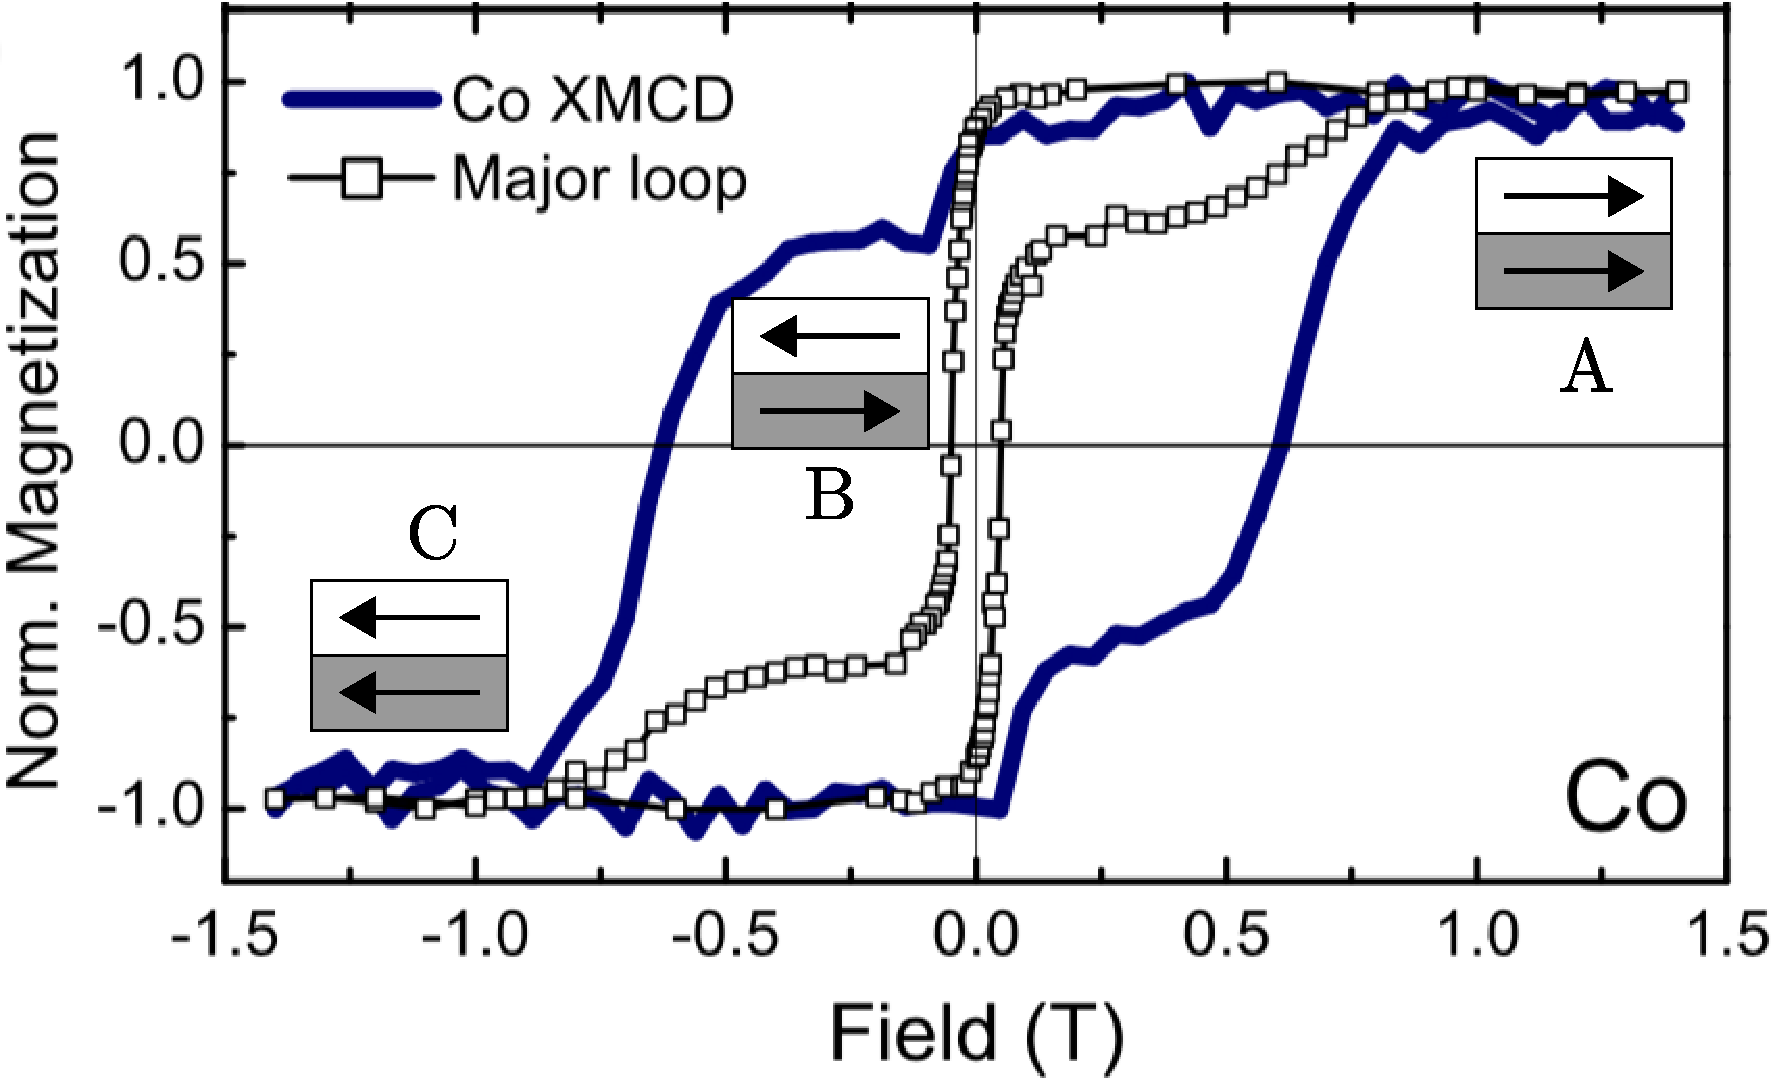
\includegraphics[width=.65\textwidth]{figures/intro/li_bilayer_loop.pdf}
    \caption[Major hysteresis loop and Co XMCD hysteresis loop for a \SI{6}{\nm} LSMO / \SI{6}{\nm} LSCO film on LSAT substrate.]{Major hysteresis loop (black) and Co XMCD hysteresis loop (blue) for a \SI{6}{\nm} LSMO / \SI{6}{\nm} LSCO film on LSAT substrate.  Arrows show directions of magnetic moments in top LSMO (white) and bottom LSCO (grey) layers.  Point A: both layers in same direction.  Point B: soft LSMO layer switches.  Point C: Hard LSCO layer switches.  From~\cite{Li2014}}
    \label{fig:LSCO_LSMO_bilayer_loops}
\end{figure}
Starting at the positive field side, the magnetization in both the LSCO and LSMO layers point in the positive direction.  
As the field is reduced, the coercive field of the soft LSMO layer is reached and its magnetization switches from positive to negative.  
The sample is now in a state where the soft layer and the hard layer are magnetized in opposite directions.  
Finally, the coercive field of the hard layer is reached and the magnetization in this layer is switched.  
The process repeats as the field is swept in the positive direction.
\end{sloppypar}
Interestingly in this bilayer system the nominally hard LSCO layer has a small volume switching coincidentally with the soft LSMO layer, as shown by element specific Co x-ray magnetic circular dichroism hysteresis loops~\cite{Li2014}.  
This curve is shown in Figure~\ref{fig:LSCO_LSMO_bilayer_loops} in blue, where the small change in normalized magnetization at low fields is indicative of a soft magnetic switching event.  
Studies show that this magnetically soft layer is the result of the formation of a thin \ce{Co^2+}-rich LSCO layer at the LSMO-LSCO interface leading to \ce{Co^2+} - \ce{Mn^4+} ferromagnetic superexchange, caused by charge transfer from the LSMO layer to the LSCO layer~\cite{Li2016}.  

Investigations into the \ce{Co^2+}-rich interfacial layer have focused on the cubic substrate LSAT which acts to suppress octahedral tilts in the bilayer stack.  
The impact of substrate-enhanced octahedral tilts on the charge transfer process, LSCO sublayer formation, and the resultant magnetic switching behavior has not been thoroughly investigated.  
The orthorhombic substrate \ce{NdGaO3} (NGO) is an ideal candidate to isolate the impact of enhanced interfacial octahedral tilts.  
\hkl(1 1 0)$_{o}$-oriented NGO substrates have an in-plane growth net that is slightly rectangular with in-plane pseudocubic lattice parameters of \SI{3.855}{\angstrom} and \SI{3.863}{\angstrom}, which is only \SI{0.2}{\percent} different on average than the \SI{3.868}{\angstrom} lattice parameter of LSAT.  
Figure~\ref{fig:ngo_lsat_comp} compares the LSAT and NGO substrates and clearly depicts the absence of octahedral tilts in LSAT compared with NGO.  
\begin{figure}[tb!]
    \centering
    \includegraphics[width=.65\textwidth]{figures/intro/LSATvsNGO.png}
    \caption[(001) LSAT compared with (110)${\mathrm{o}}$ NGO substrates]{(001) LSAT compared with (110)${\mathrm{o}}$ NGO substrates illustrating the presence of octahedral rotations in NGO, and the absence in LSAT}
    \label{fig:ngo_lsat_comp}
\end{figure}
Because the two substrates have very similar in-plane strain states  and different octahedral rotation patterns, a comparison of films  grown on the two materials provides a  way to isolate the impact of interfacial octahedral tilts.  

Single layer LSCO and LSMO show different effects when grown on NGO versus LSAT substrates.  
When LSMO is grown on an orthorhombic substrate like NGO, octahedral rotations are enhanced at the film substrate interface leading to distorted B-O-B bonds, weaker exchange interactions, and less stable magnetism when compared with the same films on LSAT substrates~\cite{Moon2014}.  
LSMO returns to a bulk-like octahedral rotation pattern after 3-5 unit cells on both substrates, attributed to Jahn-Teller symmetry breaking distortions in LSMO octahedra~\cite{He2010}.  
Because the distorted octahedral rotation pattern extends only a short distance, electronic and magnetic property degradation is only apparent in close proximity to the LSMO-NGO interface.  

Oxygen octahedra in LSCO are not Jahn-Teller active~\cite{Sundaram2009}; therefore, substrate induced octahedral tilts can persist for film thicknesses greater than \SI{17}{\nm}, as shown by transmission electron microscopy (TEM) analysis, although the magnitude of rotations changes as a function of film thickness~\cite{Byers2019}. 
This distance is an order of magnitude larger than the distance observed for LSMO films.  
In LSCO, simulations have shown that the effects of octahedral tilts from the NGO substrates and interfacial strain each act to break the $t_{2g}$ and $e_g$ orbital degeneracy resulting in fewer half full orbitals and reduced magnetization.  
Interestingly the combination of octahedral tilts and interfacial strain restores some of this degeneracy resulting in higher magnetization.  
NGO substrates induce both interfacial strain and changed octahedral tilts whereas LSAT substrates only apply interfacial strain.  
Therefore LSCO films grown on NGO substrates will have a higher magnetization than those grown on LSAT substrates~\cite{Biegalski2014}.  

TEM studies of \SI{17}{\nm} LSCO / \SI{20}{\nm} LSMO bilayers grown on LSAT substrates illustrate the importance of the order of material growth.  
When the LSMO layer is grown first (referred to as bilayer MC) octahedral tilts are nearly absent in both LSMO and LSCO layers, contrasted with bilayers where LSCO is grown first (referred to as bilayer CM) in which octahedral tilts persist throughout the entire \SI{17}{\nm} LSCO film and into the capping LSMO layer~\cite{Byers2019}.  
Such a change has consequences on the LSMO / LSCO charge transfer process: bilayer MC shows little \ce{Co^2+} ion formation and the two layers are magnetically decoupled whereas in bilayer CM, strong coupling exists between the LSCO and LSMO layers and charge transfer results in a thin interfacial LSCO layer with magnetically active \ce{Co^2+} ions, suggesting that the presence of octahedral rotations enhances the coupling between interfacial layers.  

The aforementioned studies of single layer LSMO and LSCO on NGO and LSAT substrates, as well as LSMO / LSCO bilayers on LSAT substrates, illustrate the complex interplay of degrees of freedom responsible for observed functional properties in complex oxides; however, a thorough investigation of LSMO / LSCO bilayers on NGO substrates has not been performed.  
Studying the bilayer system on NGO substrates and investigating the impact of substrate-induced octahedral  tilts on magnetic  behavior and charge transfer is the aim of this thesis.  
Chapter 2 discusses the experimental techniques required to extensively characterize oxide bilayers, Chapter 3 covers structural characterization of this system, Chapter 4 presents magnetometry and soft x-ray magnetic spectroscopy results of the bilayers including a comparison with bilayers on LSAT substrates, and Chapter 5 summarizes the presented results and proposes future research directions to pursue.  
